\beginsong{Was ließen jene}[wuw={olka (Erich Scholz), Nerother Wandervogel}, pfii={51}, bo={366}, gruen={218}]

\beginverse 
\endverse
\centering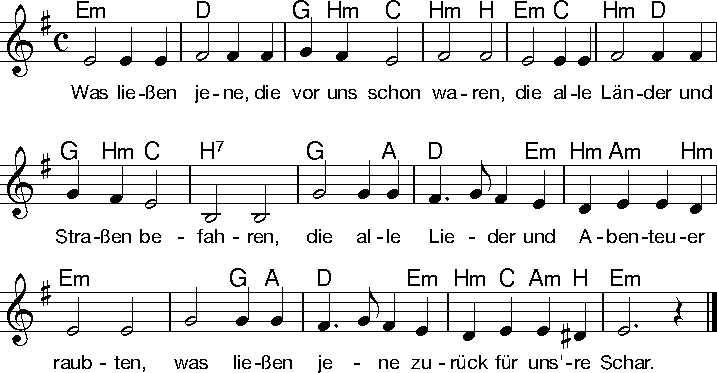
\includegraphics[width=1\textwidth]{Noten/Lied092a.pdf}

\beginverse
\[Em]Atem der \[D]Meere, Ge\[G]zei\[Hm]ten \[C]des \[Hm]Blu\[H]tes, 
\[Em]Träu\[C]me von \[Hm]Ta\[D]ten, ver\[G]lo\[Hm]cken \[C]des \[H7]Mutes, 
\[G]Lieder \[A]der \[D]Sehnsucht \[Em]und \[Hm]Rundgang \[Am]um \[Hm]die \[Em]Flammen,
Erb\[G]teil \[A]an \[D]Bildern, \[Em]be\[Hm]stäubt \[C]mit \[Am]sprö\[H]dem \[Em]Glanz.
\endverse

\beginverse
^Unter den ^Hufen der ^ja^gen^den ^Stun^den, 
^un^ter des ^Him^mels ent^hei^lig^ten ^Runden,
^Unter ^den ^Worten, ^an ^die wir ^nicht ^mehr ^glaubten,
wa^gen ^wir ^unser ^Ge^setz ^und ^un^ser ^Glück.
\endverse

\beginverse
^Heben die ^Stimmen und ^he^ben ^die ^Hän^de, 
^ste^hen ver^streut ^auf ver ^brann^tem ^Ge^lände,
^fügen ^die ^Steine ^der ^dürren ^Zeit ^zu^sammen,
bin^den ^ver^trauend ^dem ^Gott ^den ^fri^schen ^Kranz.
\endverse

\endsong
